\documentclass[12pt]{amsart}
%prepared in AMSLaTeX, under LaTeX2e
\addtolength{\oddsidemargin}{-.65in} 
\addtolength{\evensidemargin}{-.65in}
\addtolength{\topmargin}{-.55in}
\addtolength{\textwidth}{1.3in}
\addtolength{\textheight}{.9in}

\renewcommand{\baselinestretch}{1.05}

\usepackage{verbatim} % for "comment" environment

\usepackage{palatino}

\newtheorem*{thm}{Theorem}
\newtheorem*{defn}{Definition}
\newtheorem*{example}{Example}
\newtheorem*{problem}{Problem}
\newtheorem*{remark}{Remark}

\usepackage{fancyvrb,xspace,dsfont}

\usepackage[final]{graphicx}

% macros
\usepackage{amssymb}

\usepackage{hyperref}
\hypersetup{pdfauthor={Ed Bueler},
            pdfcreator={pdflatex},
            colorlinks=true,
            citecolor=blue,
            linkcolor=red,
            urlcolor=blue,
            }

\newcommand{\br}{\mathbf{r}}
\newcommand{\bv}{\mathbf{v}}
\newcommand{\bx}{\mathbf{x}}
\newcommand{\by}{\mathbf{y}}

\newcommand{\cB}{\mathcal{B}}
\newcommand{\cD}{\mathcal{D}}
\newcommand{\cF}{\mathcal{F}}
\newcommand{\cH}{\mathcal{H}}
\newcommand{\cL}{\mathcal{L}}
\newcommand{\cV}{\mathcal{V}}
\newcommand{\cW}{\mathcal{W}}

\newcommand{\CC}{\mathbb{C}}
\newcommand{\NN}{\mathbb{N}}
\newcommand{\RR}{\mathbb{R}}
\newcommand{\ZZ}{\mathbb{Z}}

\renewcommand{\Im}{\mathrm{Im}}
\renewcommand{\Re}{\mathrm{Re}}

\newcommand{\eps}{\epsilon}
\newcommand{\grad}{\nabla}
\newcommand{\lam}{\lambda}
\newcommand{\lap}{\triangle}

\newcommand{\ip}[2]{\ensuremath{\left<#1,#2\right>}}

\newcommand{\image}{\operatorname{im}}
\newcommand{\onull}{\operatorname{null}}
\newcommand{\rank}{\operatorname{rank}}
\newcommand{\range}{\operatorname{range}}
\newcommand{\trace}{\operatorname{tr}}
\newcommand{\Span}{\operatorname{span}}

\newcommand{\prob}[1]{\bigskip\noindent\textbf{#1.}\quad }

\newcommand{\pts}[1]{(\emph{#1 pts}) }
\newcommand{\epart}[1]{\medskip\noindent\textbf{(#1)}\quad }
\newcommand{\ppart}[1]{\,\textbf{(#1)}\quad }

\newcommand{\ds}{\displaystyle}

\newcommand{\nex}{\medskip\noindent}


\begin{document}
\scriptsize \noindent Math 617 Functional Analysis (Bueler) \hfill \emph{version 3; assigned 22 April 2024}
\normalsize\medskip

\Large\centerline{\textbf{Assignment 8}}
\large
\medskip

\centerline{\textbf{Due at 5:00pm on Thursday 2 May 2024}}
\medskip
\normalsize

\thispagestyle{empty}

\bigskip
\noindent This Assignment is based on sections 3.3, 3.4, 4.1, 4.2, 4.3, 5.1, 5.2, and 5.3 of our textbook.\footnote{Borthwick (2020)~\emph{Spectral Theory: Basic Concepts and Applications}, Springer.}  I recommend working backward from the major theorems in Chapter 5 to understand the material from Chapters 3 and 4 on which they depend.

\bigskip
\noindent Note that we have skipped material on compact operators (sections 3.5, 4.4).  Also we have skipped subsections 3.4.3, 4.1.3, and 4.1.4, and all later material in the book starting with section 5.4.

\medskip
\noindent \textsc{Please do the following exercises.}
\smallskip

\renewcommand{\SS}{\mathbb{S}}


% Exer 4.4, but made specific to \ell^2
\prob{P38}  \emph{The basic facts in Lemma 4.3 and Theorem 4.4 are important in this problem.  You have already shown, on the Midterm Quiz, that $R$ has no eigenvalues.}

\medskip\noindent Let $R$ be the right shift on $\cH=\ell^2$, a bounded operator:
	$$R (a_1,a_2,a_3,\dots) = (0,a_1,a_2,\dots).$$

\epart{a}  Show that $L=R^*$ is the left shift, and that $\|R\|=\|L\|=1$.

\epart{b}  Consider any $\lambda\in\CC$ such that $|\lambda|<1$.  By constructing an eigenvector, show that $\lambda$ is an eigenvalue of $L$.  (\emph{Concretely construct the eigenvector.  Observe/show that it is in $\cH$.})

\epart{c}  Find $\sigma(L)$ and $\sigma(R)$.


% Exer 4.6
\prob{P39}  \emph{By Theorem 4.15, your only job here is to show that negative real numbers are in $\rho(A)$.  One route uses Theorem 3.18, applying Lemma 3.7 to show that the relevant range is dense.}

\medskip\noindent Prove that the spectrum of a positive self-adjoint operator $A$ satisfies $\sigma(A) \subset [0,\infty)$.


% Exer 4.5
\prob{P40}  \emph{Your job is to show that any $z\in\CC\setminus \SS$ is in the resolvent set.  This can be done using only the geometric series (4.16) and (4.28).  Please do not use Theorem 5.5; one should establish $\sigma(U) \subset \SS$ first.}

\medskip\noindent Let $U$ be a unitary operator on $\cH$.  Show that $\sigma(U) \subset \SS = \{z\in\CC\,:\,|z|=1\}$.


\prob{P41}  Suppose $A$ is a self-adjoint operator on $\cH$.  Apply the (bounded Borel) functional calculus Theorem 5.9 to show that if $\rho(A)$ is nonempty and $z\in\rho(A)$ then
	$$\|(A-z)^{-1}\| = \frac{1}{\operatorname{dist}(z,\sigma(A))}.$$
(\emph{Hint. Separate the case where $z$ is strictly complex from the case where $z\in\RR$.  Construct a continuous, bounded $f$ to do the job in each case, and use (5.17).})


\clearpage\newpage
\prob{P42}  \emph{Each self-adjoint operator generates a commutative unitary group.  Again we apply the bounded Borel functional calculus.}

\medskip\noindent Let $A$ be a self-adjoint operator on $\cH$.  Suppose $t\in\RR$ and let $f_t(x) = e^{itx}$ and apply the functional calculus to define $U(t) = f_t(A) = e^{itA}$.  Show that: $U(t)$ is unitary, $U(0) = I$, and $U(t+s) = U(t) U(s)$.


% Exer 5.5
\prob{P43 (Extra Credit)}  \emph{In quantum mechanics, this calculation explains why the self-adjoint Hamiltonian operator generates unitary time-evolution, preserving total probability.}

\epart{a}  Suppose $A$ is a self-adjoint operator on $\cH$.  Let $U(t) = e^{itA}$ as in \textbf{P41}, for $t\in\RR$.  Show that for $v\in\cD(A)$,
	$$\frac{d}{dt}\Big|_{t=0} (U(t)v) = \lim_{\eps\to 0} \frac{U(\eps)v-v}{\eps} = i A v.$$

\epart{b}  Conclude that if $u_0\in\cD(A)$ then $u(t) = U(t) u_0$ solves the PDE initial-value problem $u'(t) = iAu(t)$ and $u(0)=u_0$.


\prob{P44}  \emph{The job: rigorously calculate the bound states of a square-well potential Hamiltonian using the spectral theory of self-adjoint operators and concrete solutions of linear ODEs.  To see the significance, compare what happens in section 7.4.}

\epart{a}  For $L>0$ define the function of $x\in\RR$ which is graphed in the left figure:
	$$V_L(x) = \begin{cases} 0, & |x|>1, \\ -L, & |x|<1. \end{cases}$$
(\emph{The values $V_L(\pm 1)$ affect no results.})  Let $\cH=L^2(\RR)$.  Show that the multiplication operator $M = M_{V_L}\in\cL(\cH)$ is self-adjoint and satisfies $\|M\|=L$.

\bigskip
\begin{center}
\mbox{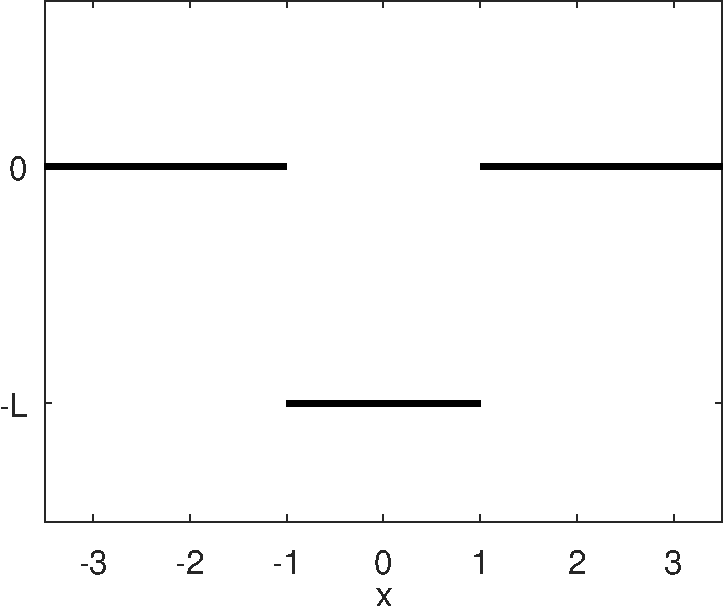
\includegraphics[height=60mm]{figs/squarepot.pdf} \hspace{10mm} 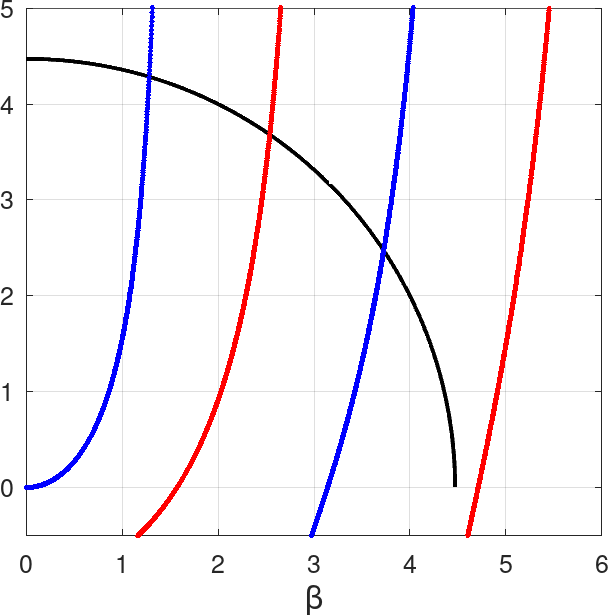
\includegraphics[height=60mm]{figs/squareeigs.png}}
\end{center}

\medskip
\epart{b}  Example 3.23 (page 49) shows $A = -d^2/dx^2$ is self-adjoint on domain $\cD(A)=H^2(\RR)\subset\cH$, the Sobolev space defined in section 2.5 and, via Fourier transform, on page 37.  Given this, show that
	$$H=-\frac{d^2}{dx^2} + V_L(x) = A + M$$
is a self-adjoint unbounded operator with the same domain $\cD(H)=\cD(A)$.

\epart{c}  Now consider the eigenfunctions (eigenvectors) of $H$; we will see below that they exist.  Suppose $Hu=\lambda u$ for nonzero $u\in\cD(H)=H^2(\RR)$ and $\lambda\in\RR$.  From the statement of Theorem 2.26, explain why $u\in C^1(\RR)$.  (\emph{This is a straightforward reading.})

\epart{d}  Consider negative eigenvalues of $H$.  Let $\lambda=-\alpha^2$ for $\alpha > 0$.  Observe that if $Hu=\lambda u$ for nonzero $u\in\cD(H)$ then $u(x)$ will have the following properties: square-integrable, continuous, and first derivative is continuous.  Furthermore it satisfies a constant-coefficient, linear ODE on each interval where $V_L(x)$ is constant; show that
    $$u(x) = \begin{cases}
                a_1 e^{-\alpha x} + a_2 e^{\alpha x}, & -\infty < x < -1 \\
                b_1 \cos(\beta x) + b_2 \sin(\beta x), & -1 < x < 1 \\
                c_1 e^{-\alpha x} + c_2 e^{\alpha x}, & 1 < x < \infty
             \end{cases}$$
where $\alpha^2+\beta^2=L^2$.  Turn the known properties of $u(x)$ into facts about the coefficients $a_i,b_i,c_i$.

\epart{e}  Consider eigenfunctions $u(x)$ which are even in $x$, and real-valued.  Show that the conditions on $u(x)$ imply that
	$$\sqrt{L^2-\beta^2} = \beta \tan(\beta).$$
(\emph{The solutions of this transcendental equation in $\beta$ can be identified graphically: the quarter circle $y=\sqrt{L^2-\beta^2}$ and the graph $y=\beta \tan(\beta)$ intersect.  See the right figure above, for $L=20$.  Even eigenfunctions correspond to black and blue intersections.})

\epart{f}  Consider eigenfunctions $u(x)$ which are odd in $x$, and real-valued.  Derive the corresponding equation for $\beta$, where again $\alpha^2+\beta^2=L^2$.  (\emph{In the right figure above,the black and red curves intersect for odd eigenfunctions.})

\epart{g}  How many negative eigenvalues does $H$ have when $L=44$?  You will need to generate an adequately-accurate graph to answer this.

\medskip
\epart{Extra Credit A}  Use numerical means to find the values of each eigenvalue in part \textbf{(g)} accurate to 10 digits.  (\emph{Graphing is recommended to get initial eigenvalue iterates.})  Graph the corresponding eigenfunctions.

\epart{Extra Credit B}  It is known that there are no eigenvalues $\lambda>0$ of $H$.  However, for any positive $\lambda$, construct an approximate eigenvalue in the sense of Theorem 4.16.  That is, construct an approximate eigenfunction sequence.  (\emph{These are the \emph{scattering states} of the quantum system.})

\end{document}
